
\begin{figure}[H]
\centering
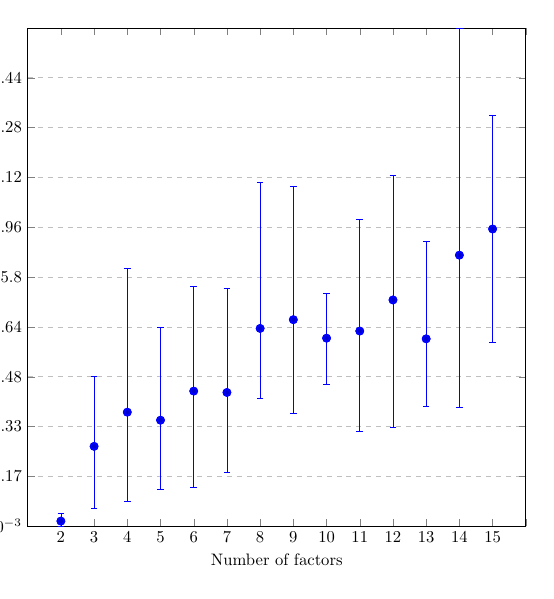
\begin{tikzpicture}[scale=0.6, trim axis left, trim axis right]
\begin{axis}[
    width=1\textwidth,
    height=1\textwidth,
    xlabel={Number of factors},
    ylabel={Time taken (s)},
    xmin=1.0, xmax=16.0,
    ymin=0.006143, ymax=11.600464,
    xticklabels={2, 3, 4, 5, 6, 7, 8, 9, 10, 11, 12, 13, 14, 15,},
    xtick={2, 3, 4, 5, 6, 7, 8, 9, 10, 11, 12, 13, 14, 15, 16, 17, 18, 19, 20},
    ytick={0.006143, 1.1655751, 2.3250072, 3.4844393, 4.6438714, 5.8033035, 6.9627356, 8.1221677, 9.2815998, 10.4410319},
    ymajorgrids=true,
    grid style=dashed,
]

\addplot+[
    blue,
    very thick,
    forget plot,
    only marks
    ]
    plot[
    very thick,
    error bars/.cd,
    y dir=plus,
    y explicit
    ]
    table[x=x,y=y,y error expr=\thisrow{y-max}] {
    x    y    y-max
    11	4.5472213	2.5943217
10	4.3813821	1.0425829
13	4.3661165	2.2646215
12	5.2711618	2.8968452
15	6.9222887	2.6438803
14	6.3138906	5.2865734
3	1.863128	1.640782
2	0.1234448	0.1778742
5	2.4723056	2.1704004
4	2.6590272	3.3385778
7	3.117723	2.416449
6	3.1491498	2.4300842
9	4.8116204	3.1010296
8	4.608257	3.398077

    };

\addplot+[
    blue,
    very thick,
    forget plot,
    only marks
    ]
    plot[
    very thick,
    error bars/.cd,
    y dir=plus,
    y explicit
    ]
    table[x=x,y=y,y error expr=\thisrow{y-min}] {
    x    y    y-min
    11	4.5472213	-2.3403543
10	4.3813821	-1.0745521
13	4.3661165	-1.5725185
12	5.2711618	-2.9638238
15	6.9222887	-2.6459547
14	6.3138906	-3.5397636
3	1.863128	-1.432919
2	0.1234448	-0.1173018
5	2.4723056	-1.6200266
4	2.6590272	-2.0718492
7	3.117723	-1.859811
6	3.1491498	-2.2341108
9	4.8116204	-2.1788084
8	4.608257	-1.617636

    };

\end{axis}
\end{tikzpicture}
\vspace{-0.3cm}
\caption{Large primes, Iterations: $\sqrt{n}$ }\label{fig:LenstrasEllipticCurveFactorizationlargeprimes(maximumIterations:-1)factors}
\end{figure}

